\documentclass[11pt,a4paper]{article}
% rozmery stranky
\usepackage[left=1.5cm,text={18cm, 25cm},top=2.5cm]{geometry}
% cestina a fonty
\usepackage[czech]{babel}
\usepackage[utf8]{inputenc}
\usepackage[T1]{fontenc}
% dalsi balicky
\usepackage{graphicx}
\usepackage{enumitem}
\usepackage{indentfirst}
\usepackage{url}
\usepackage[bookmarksopen,colorlinks,plainpages=false,urlcolor=blue,
unicode,linkcolor=black]{hyperref}


\begin{document}

  \begin{titlepage}
    \begin{center}
      \Huge
      \textsc{Fakulta informačních technologií \\ Vysoké učení technické v~Brně}
      \vspace{100px}
      \begin{figure}[!h]
        \centering
        
\includegraphics[height=5cm]{logo}
      \end{figure}
      \\[50mm]
      \LARGE{Tvorba uživatelských rozhraní \,--\, projekt č. 93 \\
             Správa hostingu}
      \vfill
    \end{center}
    \Large{Roman Blanco (xblanc01) - kapitán týmu \hfill 24.11.2014 \\
           Adam Jež (xjezad00)}

  \end{titlepage}

  \section{Abstrakt}

    Cílem zadaného projektu je navrhnout a vytvořit uživatelské rozhraní,
    umožňující uživateli konfigurovat a spravovat své hostingové služby.
    Námi navržené rozhraní by mělo umožňovat správu FTP účtů, DNS
    záznamů, e-mailů a MySQL databází. Ovládání rozhraní navrhujeme tak, aby
    bylo přizpůsobeno jak uživatelům stolních počítačů, tak i uživatelům
    mobilních zařízení, které dokáží zobrazit internetový obsah. Protože naší
    snahou je maximální komfort zákazníků, nejčastěji užívané úkony by měly
    být lehce a rychle proveditelné.

  \section{Úvod}

    V~současnosti již existuje mnoho řešení uživatelských rozhraní pro správu
    hostingu.

    Při vyhledávání inspiračního materiálu jsme se zaměřili na vlastní práci
    s~rozhraním - přehledost obsahu, způsob práce s~daty a jejich řazení.
    Při návrhu vlastního rozhraní jsme se snažili vyvarovat případných chyb,
    které jsme nalézali v~existujících řešeních. Z~tohoto hlediska nám
    materiál poskytl jak pozitivní, tak i negativní inspiraci.  Jako studijní
    materiál nám sloužilo především rozhraní webhostingů roští.cz a wedos.cz \\
    \begin{figure}[ht]
      \begin{center}
        \includegraphics[width=12cm]{rosti}
        \caption{Uživatelské rozhraní webhostingu roští.cz}
      \end{center}
    \end{figure}
    \begin{figure}[ht]
      \begin{center}
        \includegraphics[width=12cm]{wedos}
        \caption{Uživatelské rozhraní webhostingu wedos.cz}
      \end{center}
    \end{figure}

  \section{Studium}

    Pro projekt plánujeme použít tyto technologie:
    \begin{description}
      \item[bower] technologie umožňující správu javascriptových knihoven
      \item[less] preprocesor pro CSS
      \item[charts.js] knihovna umožňující jednoduché vytváření grafů
      \item[MySQL] dotazovací jazyk pro získání informací spojené s~uživatelem
      \item[PHP] skriptovací jazyk běžně používaný pro programování
                   dynamických webových stránek
      \item[XML] značkovací jazyk pro popis dokumentu
      \item[XSL] jazyk pro vyjádření stylu
    \end{description}

  %\section{Návrh aplikace}

  \section{Návrh uživatelského rozhraní}

    Našim uživatelským rozhraním bychom chtěli zaujmout také amatérské
    klienty či zákazníky z~menších firem. Oslovit se je budeme snažit
    hlavně jednoduchým a uživatelsky příjemným prostředím se základními
    funkcemi. Naše uživatelské rozhraní by mělo být natolik přívětivé, aby
    jej dokázali ovládat a spravovat i méně zkušení klienti či přímo laici.
    Předpokládáme, že naše cílová skupina nebude zkušena natolik, aby si
    vytvořila vlastní analyzační nástroje, a proto chceme dát možnost použít,
    mimo jiné, užitečné statistiky související s~navštěvováním a používáním
    hostovaných webových stránek.

  \section{Realizace}

    Dosavadní práci na projektu jsme si rozdělili následujícím způsobem:
    \begin{description}
      \item[Roman Blanco] \hfill
        \begin{itemize}
          \item návrh vzhledu rozhraní
          \item zvážení technologií pro použití
          \item vyhledání a nastudování inspiračního materiálu
        \end{itemize}
      \item[Adam Jež:] \hfill
        \begin{itemize}
          \item návrh jednotlivých částí rozhraní
          \item návrh a vytvoření ERD podle návrhu rozhraní
          \item implementace logiky aplikace
        \end{itemize}
    \end{description}

    Klíčovou vlastností administrace webhostingu by měla být přehlednost.
    Snažili jsme se vytvořit prostředí tak, aby obsahovalo pouze potřebné
    prvky a neodvádělo pozornost uživatele k~částem, se kterými v~daném úkonu
    není třeba pracovat.

    K~vytvoření přehledného prostředí jsme využili možnosti CSS/JS knihovny
    Twitter Bootstrap na všech vytvořených stránkách.
    Pro lepší znázornění dat jsme také, na stránce obsahující statistiky,
    použili JavaScriptovou knihovnu charts.js, která vytváří pohledné
    interaktivní grafy.

    Námi vytvořená administrace webhosingu obsahuje 4 hlavní části pro řízení
    webhostingu \,--\, sekce pro správu FTP účtů, emailových schránek, MySQL
    databází a DNS záznamů. Další části jsou již zmíněné statistiky,
    s~informacemi o~uživatelích navštěvující hostovaný web. Vlastníkovi
    hostingu tyto informace mohou posloužit například k~optimalizaci svého
    obsahu pro získání vyšší návštěvnosti.

    Poslední částí administrace webhostingu je sekce s~nastavením, kde lze
    měnit přihlašovací údaje a notifikace systému, ale také zakoupit či
    prodloužit služby hostingu nebo získat podrobnější informace o~již
    zakoupených službách.

    \subsection{Dosavadní implementace}

      Kostra webových stránek je připravena. Jednotlivé sekce, včetně
      stránky s~přihlašováním jsou obsahově a funkčně hotové.
      Předpokládáme, že tyto části čekají už jen mírné kosmetické
      úpravy. Je potřeba se rozhodnout, co v~zadání znamená pokyn vytvořit
      přepínání mezi více hostovanými doménami. Musíme si ujasnit, jakým
      způsobem implementovat tuto funkci.

      V~projektu aktuálně využíváme následující technologie:
      \begin{description}
        \item[charts.js] knihovna umožňující jednoduché vytváření grafů
        \item[AngularJS] knihovna umožňující vytváření interaktivnějších
                         stránek
        \item[Twitter Bootstrap] JS/CSS framework pro urychlení a usnadnění
                                 vytváření vzhledu
        \item[BootstrapValidator] knihovna pro vytvareni interaktivnich
                                  formularu
        \item[MySQL] dotazovací jazyk pro získání informací spojené
                     s~uživatelem
        \item[PHP] skriptovací jazyk běžně používaný pro programování
                   dynamických webových stránek
        \item[HTML] značkovací jazyk pro popis webovych stranek
        \item[CSS] jazyk definujici vzhled HTML elementu
        \item[XML] značkovací jazyk pro popis dokumentu
        \item[XSL] jazyk pro vyjádření stylu
      \end{description}

  \section{Testování}

    Dosavadní testování bylo prováděno pouze v~rámci týmu. Následující
    závěrečné testování rozdělíme do dvou částí.

    První část se skládá z~vytvoření dotazníku,
    který bude obsahovat taktéž úkoly pro dotazované. Dotazník pošleme širší
    skupině převážně studentů (jelikož jsme se na ně při vývoji zaměřili).
    Dotazník bude obsahovat otázky:

    \begin{itemize}
      \item Kolik je vám let?
      \item Jste studentem?
      \item Využíváte nějakých hostingových služeb, připadně jakých? Co vas
            zaujalo na první pohled?
    \end{itemize}

    Následuje řada úkonů

    \begin{itemize}
      \item Jaký máte z~webhostingu pocit?
      \item Cítil jste se v~nějakou chvíli ztracený?
      \item Měl jste s~něčím v~nějakou chvíli problém?
      \item Ohodnoťte, prosím, jak jste spokojený s~webhostingem
      \item Ohodnoťte, prosím vzhled webhostingu.
        \item Dokázal byste takovýto system používat?
      \item Napadá vás, co by se dalo zlepšit?
    \end{itemize}

    Druhá část se skládá z~osobního přístupu k~dotazovaným. Hlavním přínosem
    tohoto přístupu shledáváme v~podrobnějším výstupu takovýchto testů.
    Budou probíhat obdobně jako předchozí, s~rozdílem, že zadavatel testu bude
    měřit trvání jednotlivých úkon a sledovat, kde uživatel upírá svůj pohled,
    zda nepřehlíží důležité části navigace, nebo zda se nedostal do bodu, kde
    by si se ztratil

    Očekáváme, že výsledky testů nám potvrdí úspěch našich počátečních cílů.
    Zaměřili jsme se na jednoduchost, rychlost a přehlednost. Rádi bychom
    tedy, kdyby byl uživatel se systémem spokojený, na pohled se mu líbil
    a práce s~ním byla dostatečně efektivní a rychlá.
    Jelikož jsme použili minimum prvků, očekáváme také, že si uživatel rychle
    na systém zvykne a navigace v~něm mu nebude dělat problém.

  \section{Výsledky testů}

    Našim testem uživatelského rozhraní jsme nechali projít patnáct osob ve
    věkové kategorii od 16 do 40 let. Z~toho 10 z~nich byli studenti středních
    nebo vysokých škol.

    Většina dotazovaných uvedla že webhostingové služby nevyužívají a pro
    správné pochopení uživatelského rozhraní bylo potřeba vysvětlit technické
    pojmy použité v~námi implementovaném prostředí.
    Hostingové služby využívali z~dotazovaných pouze 3 studenti. Ti uvedli, že
    rozhraní je oproti službě kterou používají přehlednější a jednodušší.

    Pocit z~uživatelského prostředí byl u~dotazovaných vcelku pozitivní.
    Mnozí uvedli že jednoduchost je pro ně přínosem. Některým osobám se zdálo
    že postrádají nějakou funkci, kterou by zřejmě objevili při dlouhodobějším
    používání

    Většina z~dotazovaných měla problém s~porozumněním technickým výrazům,
    například u~správy FTP účtů (obrázek č. \ref{sprava-ftp}) nebo nastavení
    DNS záznamů (obrázek č. \ref{nastaveni-dns}), a ocenila by krátké
    vysvětlení pro lajky. Stránky se statisktikami
    (obrázek č. \ref{statistiky}) nebo editace emailových schránek
    (obrázek č. \ref{nastaveni-email}) byly srozumitelné všem.

    Z~pohledu grafického designu byly ohlasy kladné, s~několika poznámkami.
    Například u~nastavení účtu někteří z~dotazovaných přehlédli záložku
    pro nastavení služeb (obrázek č. \ref{nastaveni-sluzeb}), nebo také
    tlačítka pro vypnutí notifikací (obrázek č. \ref{nastaveni-uctu}) nebyly
    na první pohled příliš zřejmé.

    Až na tyto výjimky se tedy prostředí vcelku zdálo všem reálně použitelné a
    byli s~ním spokojeni. Pro reálné použití by tedy bylo vhodné doladit
    grafický design jednotlivých stránek a přidat krátké vysvětlení pro lajky
    na stránkách s~odbornějšími termíny.

  \section{Závěr}

    Přínosem z~testování je pro nás zpětná vazba, díky které víme, jaké
    nedokonalosti by bylo potřeba pro reálné použití vyřešit. Také jsme se
    dozvěděli, že rozhraní bylo přehledné a jednoduchost uživatelům vyhovovala,
    což bylo našim cílem.

  \section{Reference}

    \begin{enumerate}[label={[\arabic*]}]
      \item repoziář administrace serveru \href{https://github.com/creckx/pcp}
                                               {roští.cz}
      \item administrace serveru \href{https://wedos.cz}{wedos.cz}
    \end{enumerate}

  \appendix
  \newpage

  \section{Přílohy}

    \subsection{ERD}

      \begin{figure}[ht]
        \begin{center}
          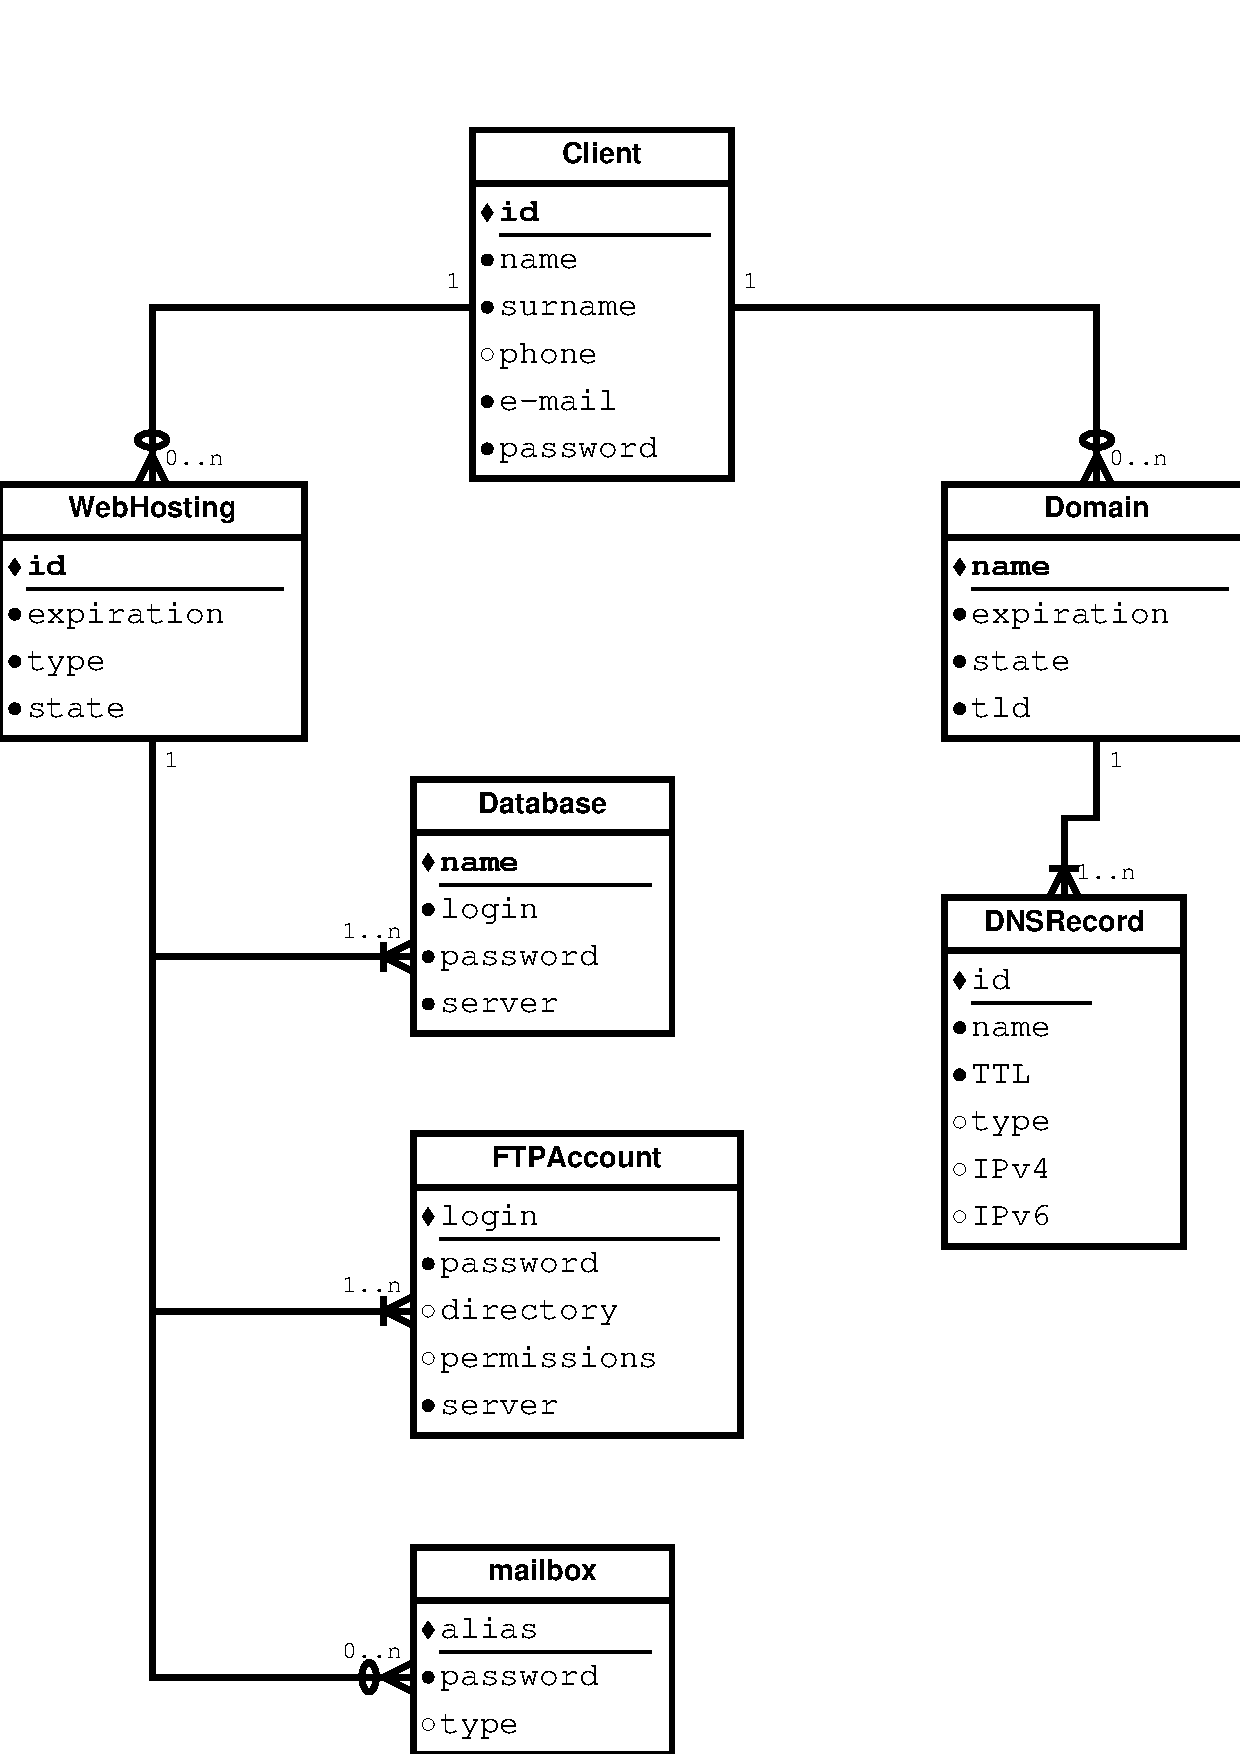
\includegraphics[width=10cm]{erd}
          \caption{ERD}
        \end{center}
      \end{figure}

    \subsection{Ukázky z~administrace}

      \begin{figure}[ht]
        \begin{center}
          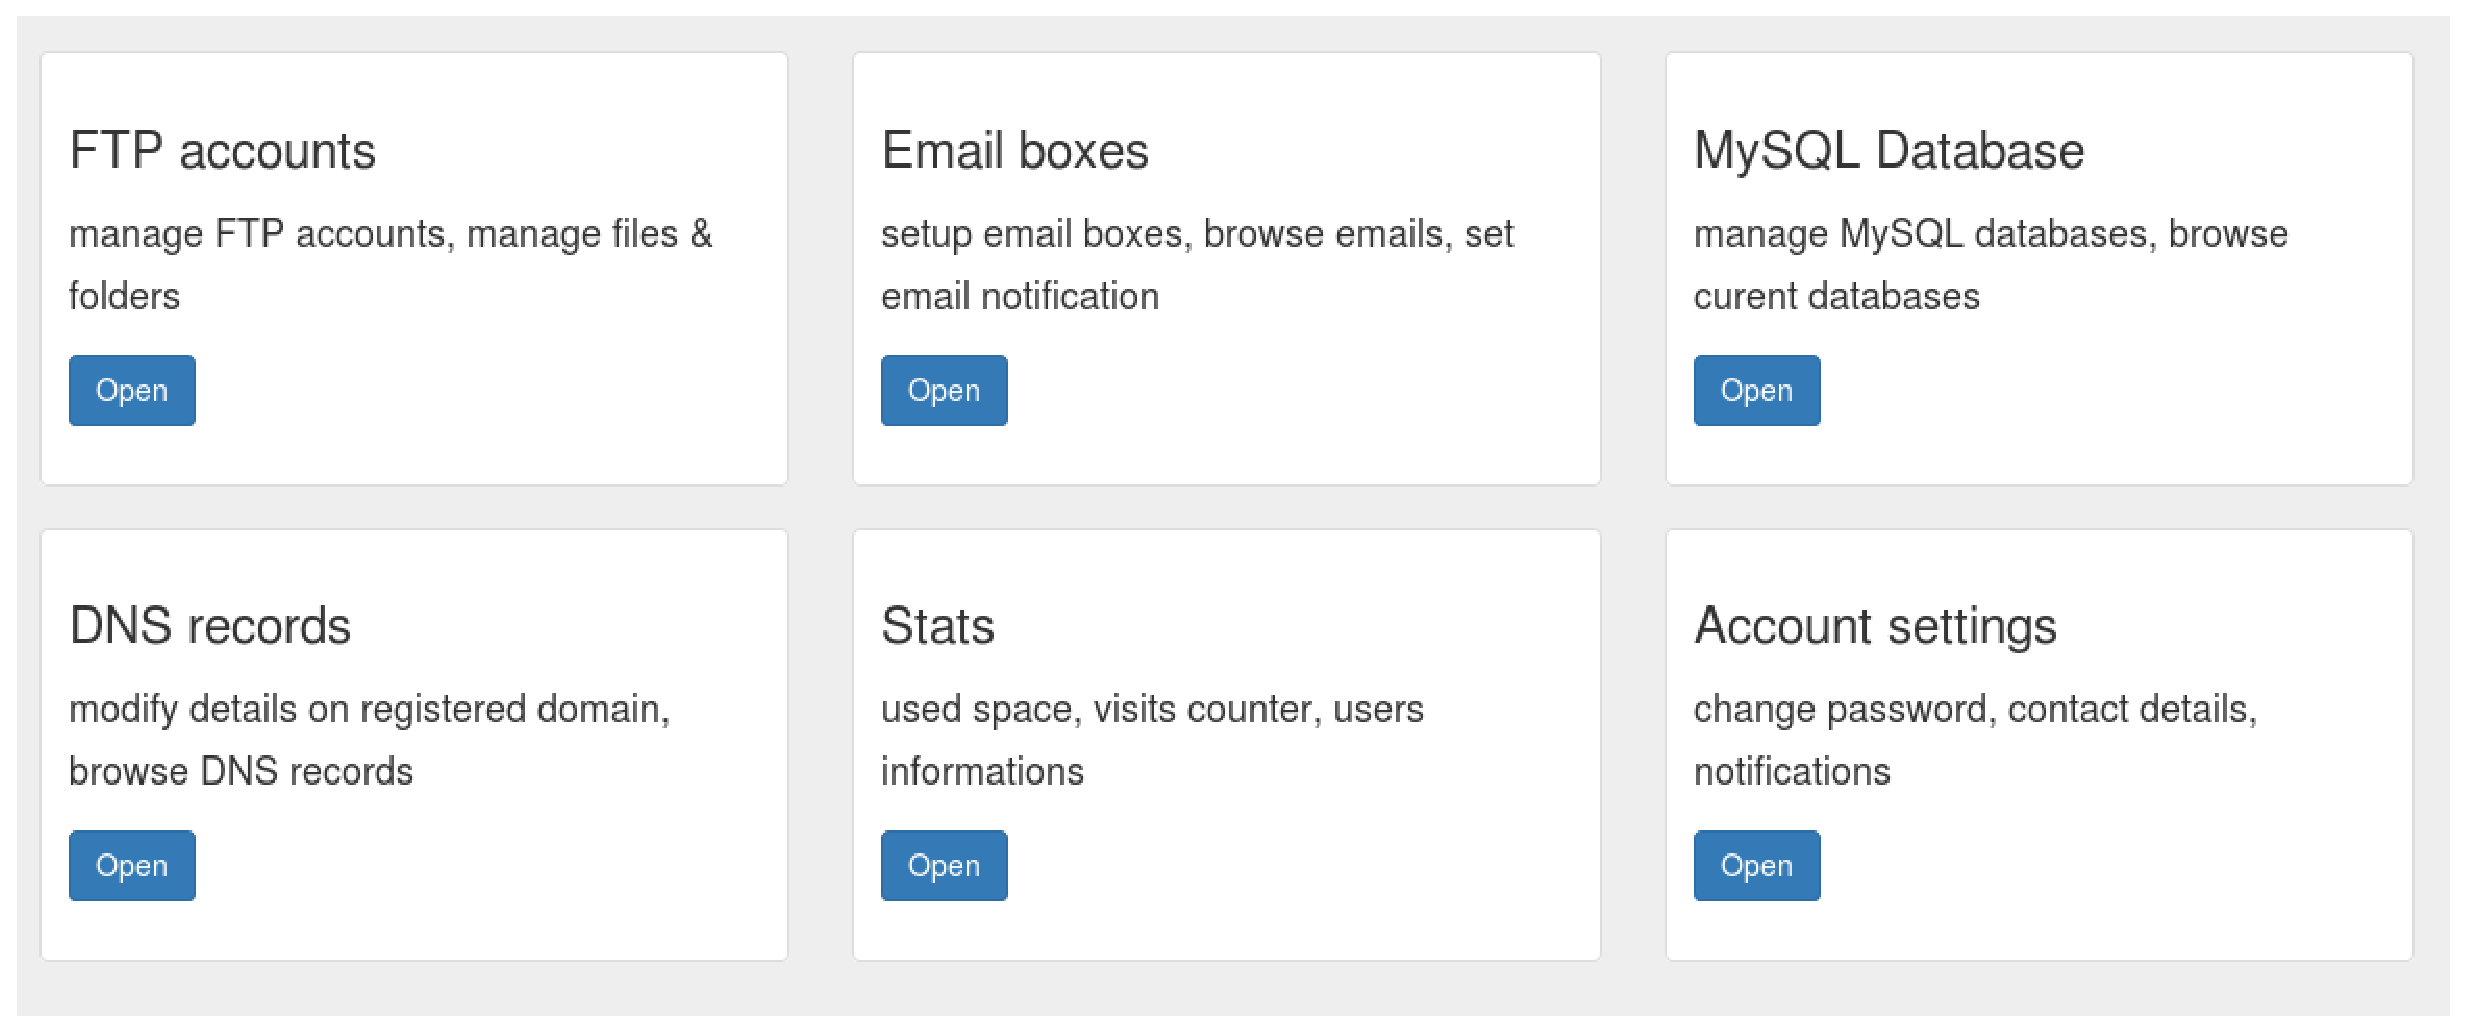
\includegraphics[width=10cm]{dashboard}
          \caption{rozcestí}
        \end{center}
      \end{figure}

      \begin{figure}[ht]
        \begin{center}
          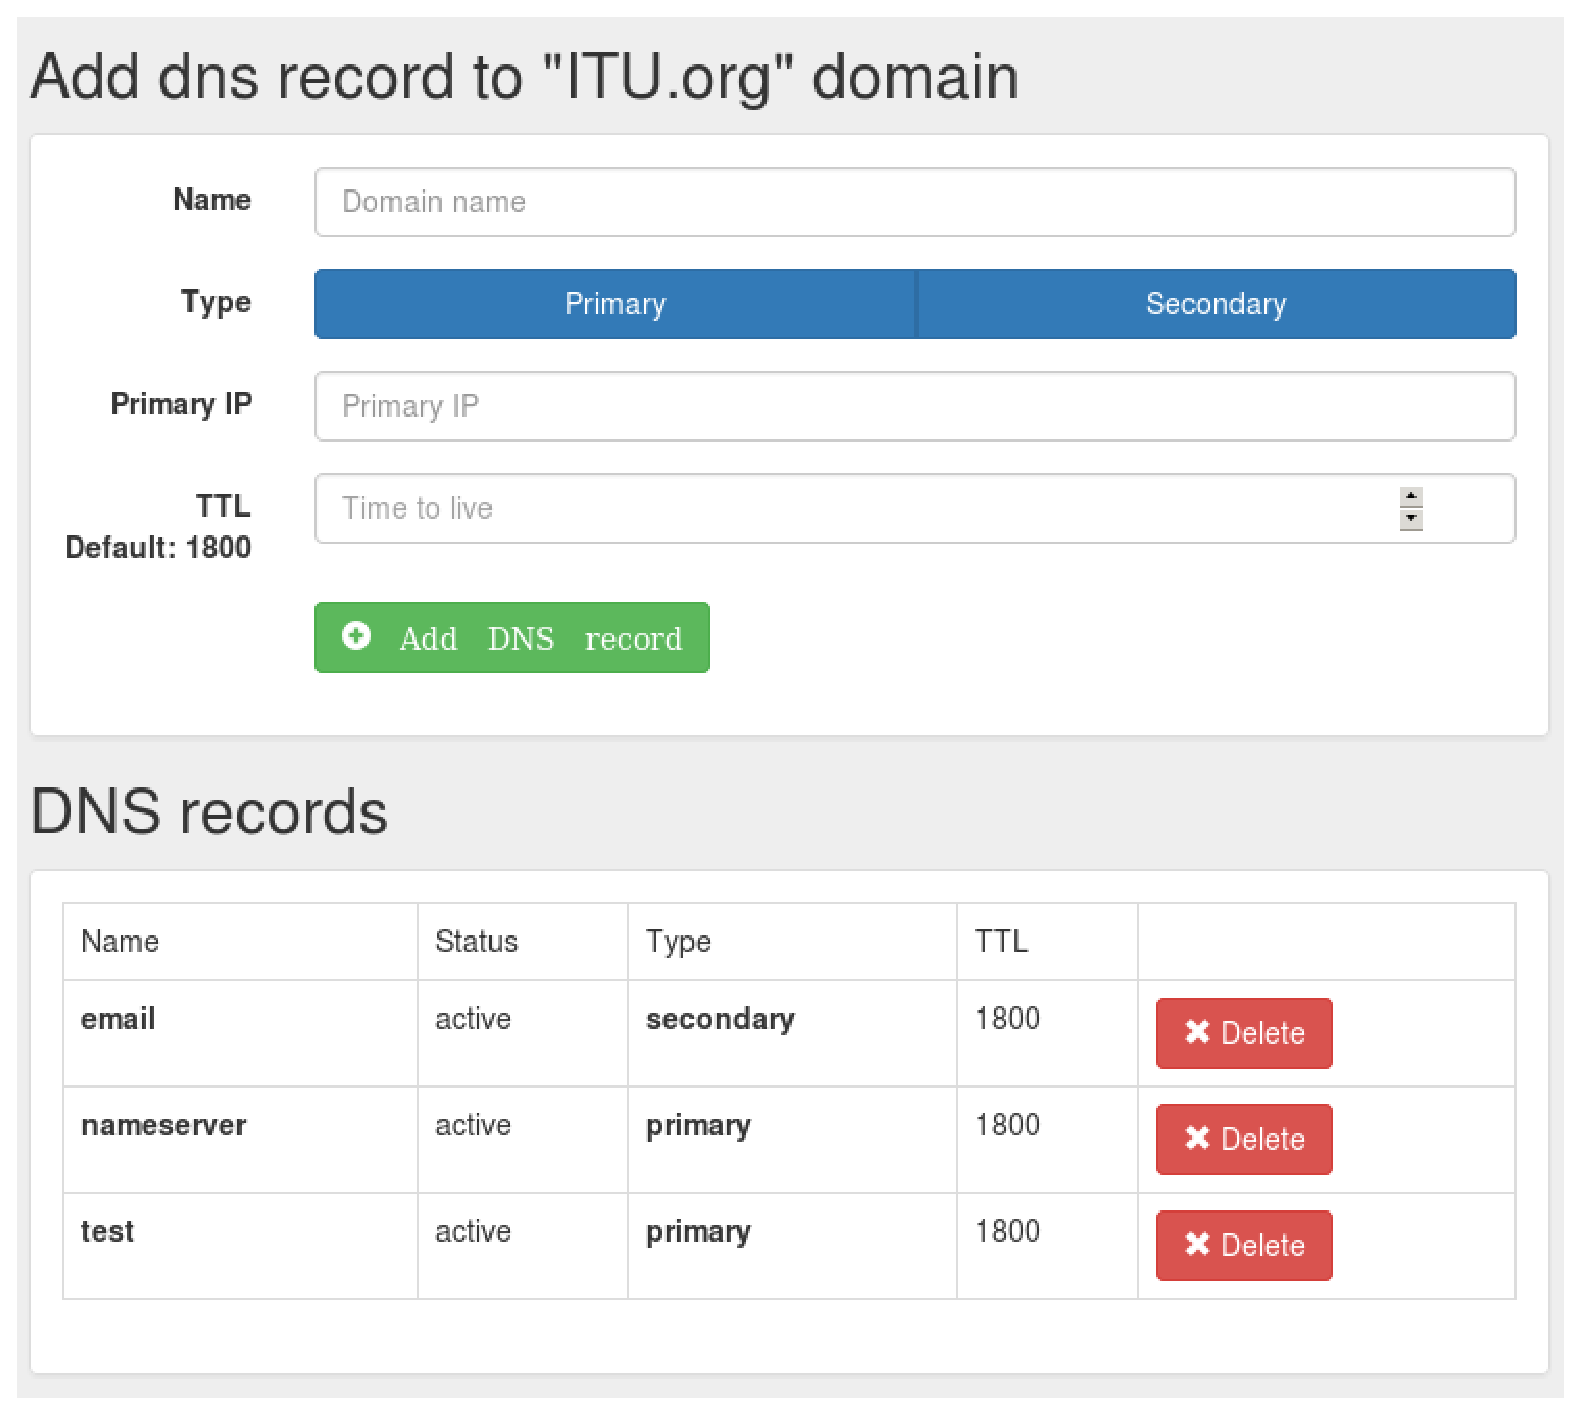
\includegraphics[width=10cm]{dns}
          \caption{nastavení DNS záznamů}
          \label{nastaveni-dns}
        \end{center}
      \end{figure}

      \begin{figure}[ht]
        \begin{center}
          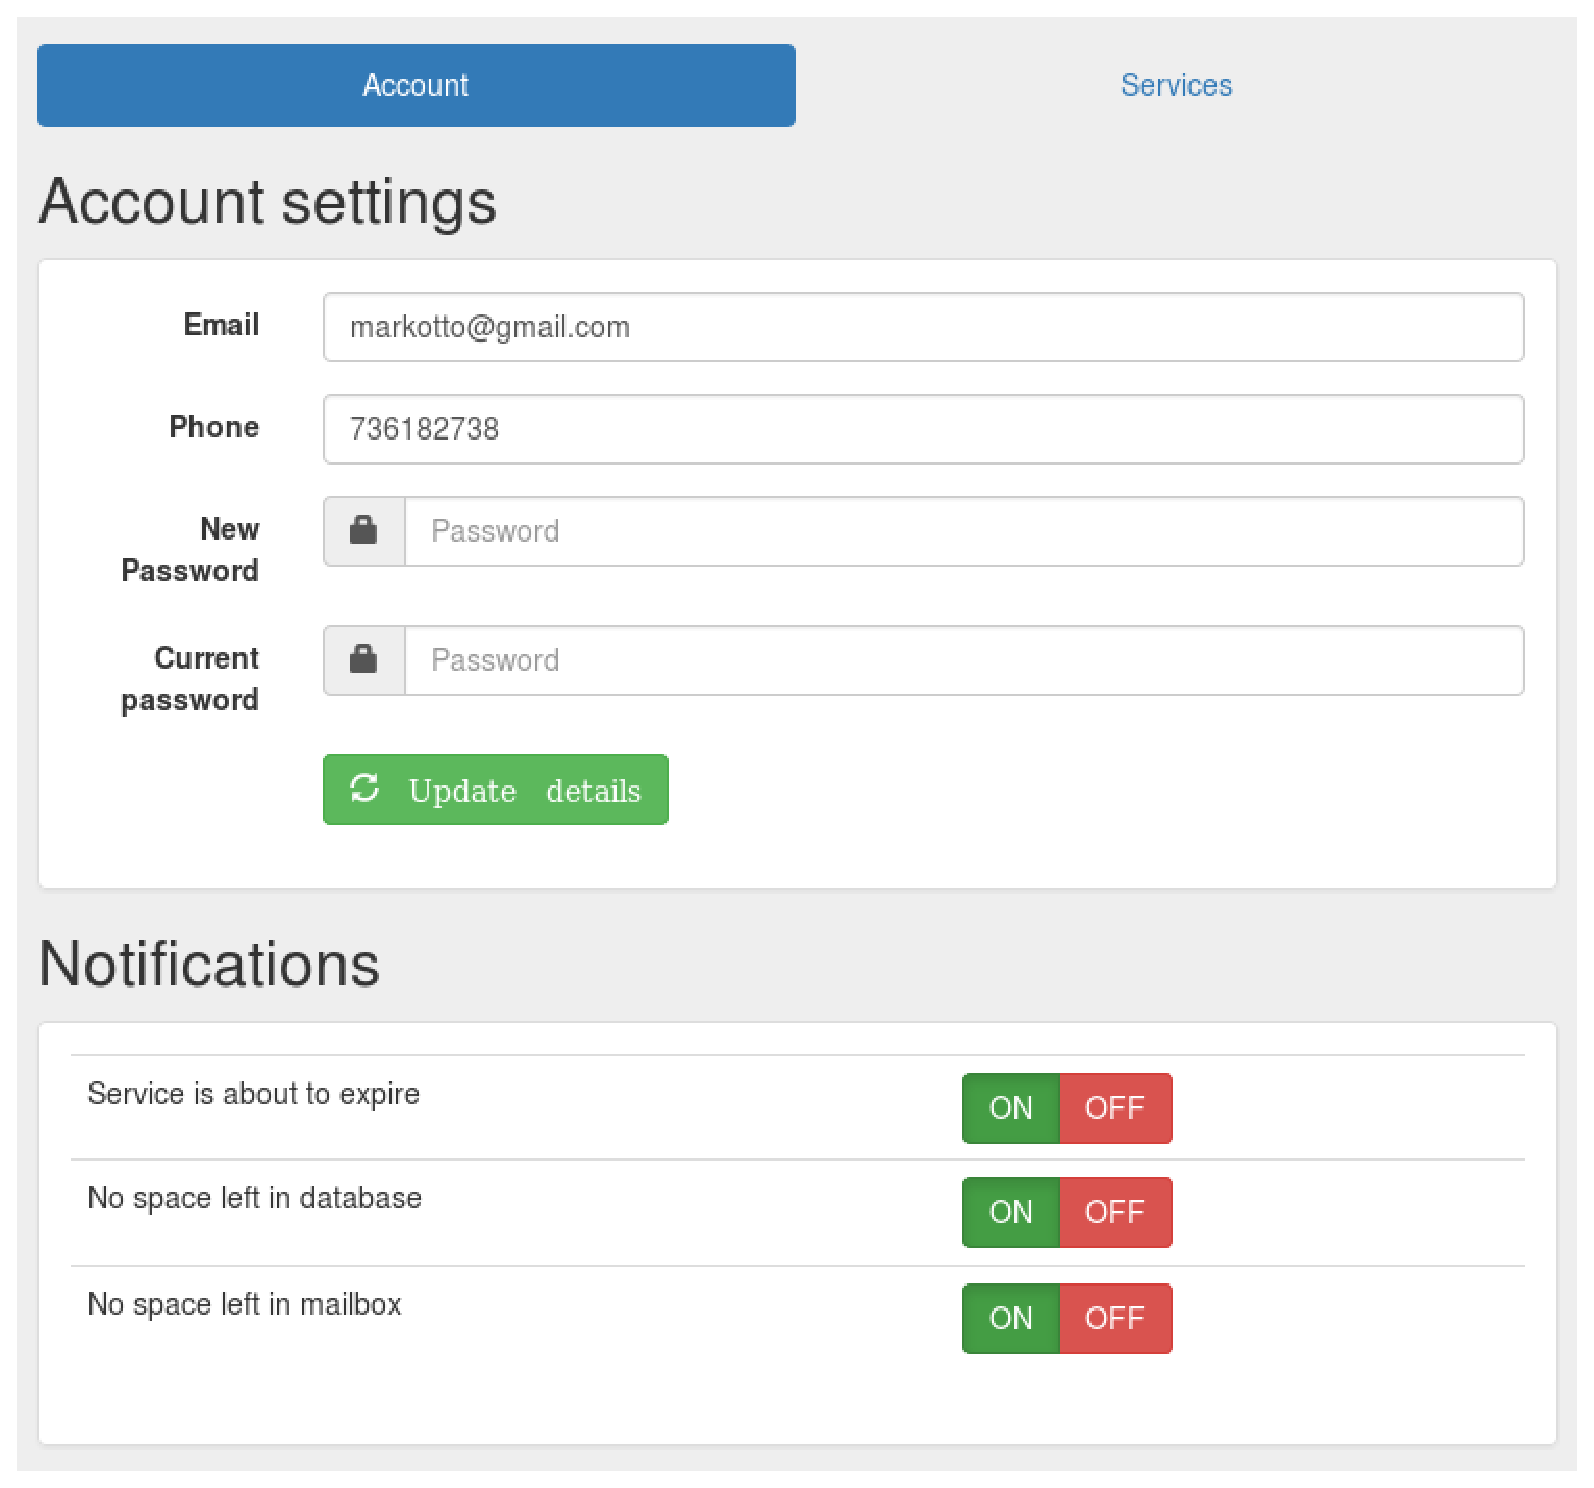
\includegraphics[width=10cm]{acc}
          \caption{nastavení uživatelského účtu}
          \label{nastaveni-uctu}
        \end{center}
      \end{figure}

      \begin{figure}[ht]
        \begin{center}
          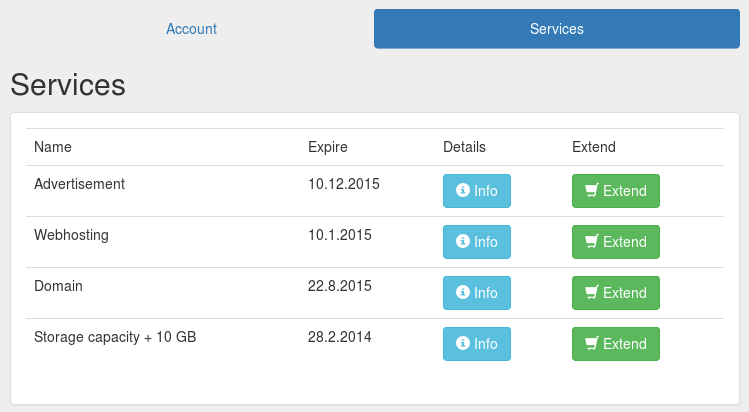
\includegraphics[width=10cm]{srvc}
          \caption{nastavení služeb}
          \label{nastaveni-sluzeb}
        \end{center}
      \end{figure}

      \begin{figure}[ht]
        \begin{center}
          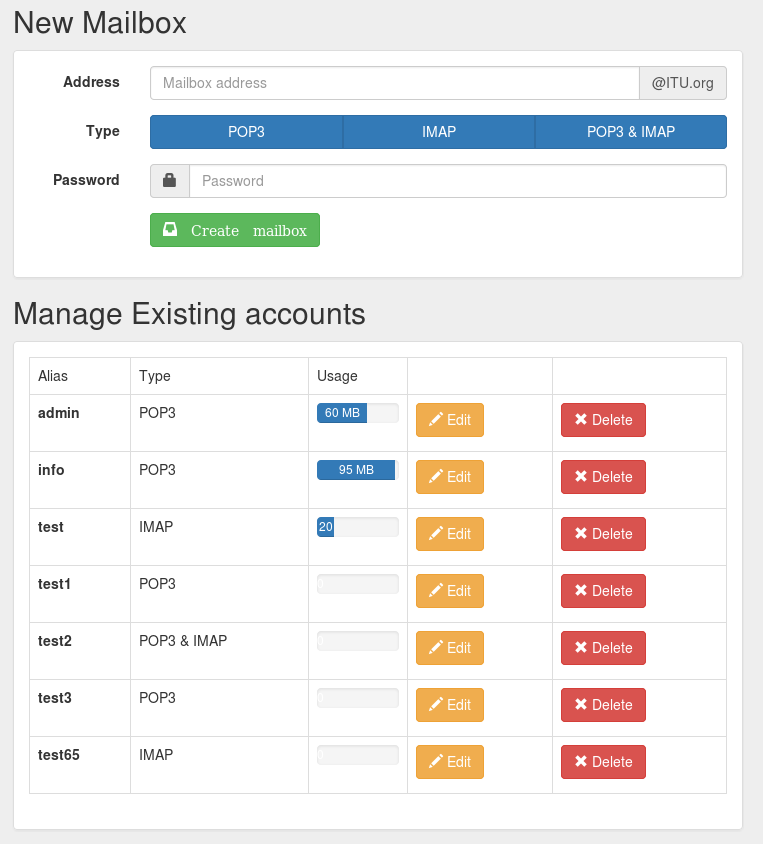
\includegraphics[width=10cm]{email}
          \caption{nastavení emalové schránky}
          \label{nastaveni-email}
        \end{center}
      \end{figure}

      \begin{figure}[ht]
        \begin{center}
          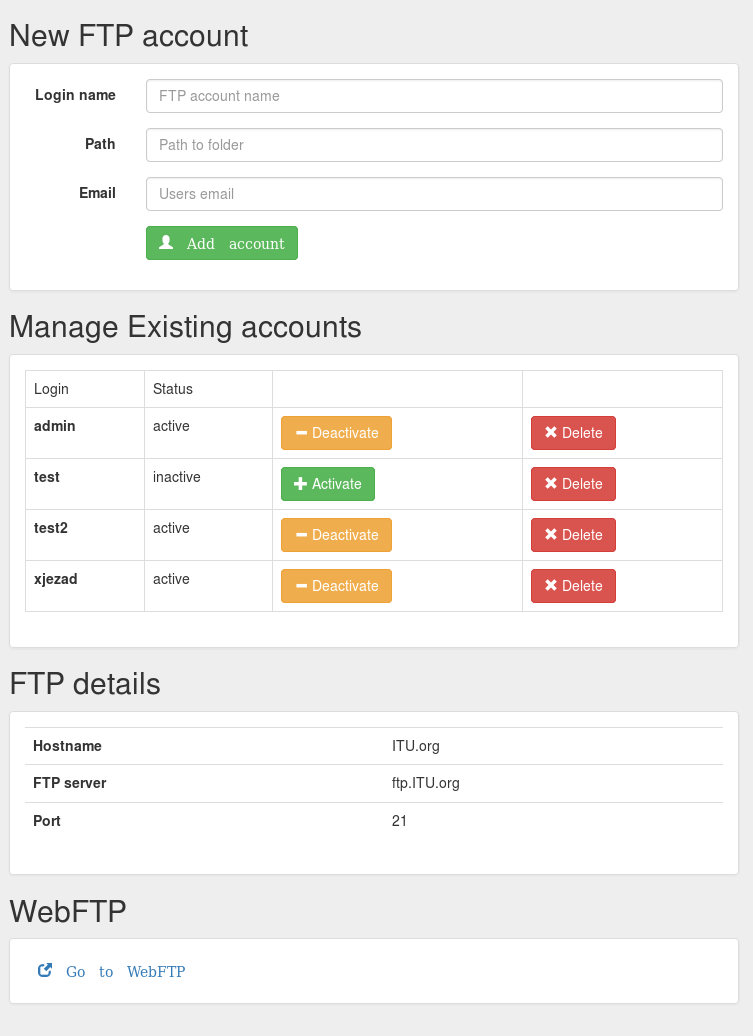
\includegraphics[width=10cm]{ftp}
          \caption{nastavení FTP účtů}
          \label{sprava-ftp}
        \end{center}
      \end{figure}

      \begin{figure}[ht]
        \begin{center}
          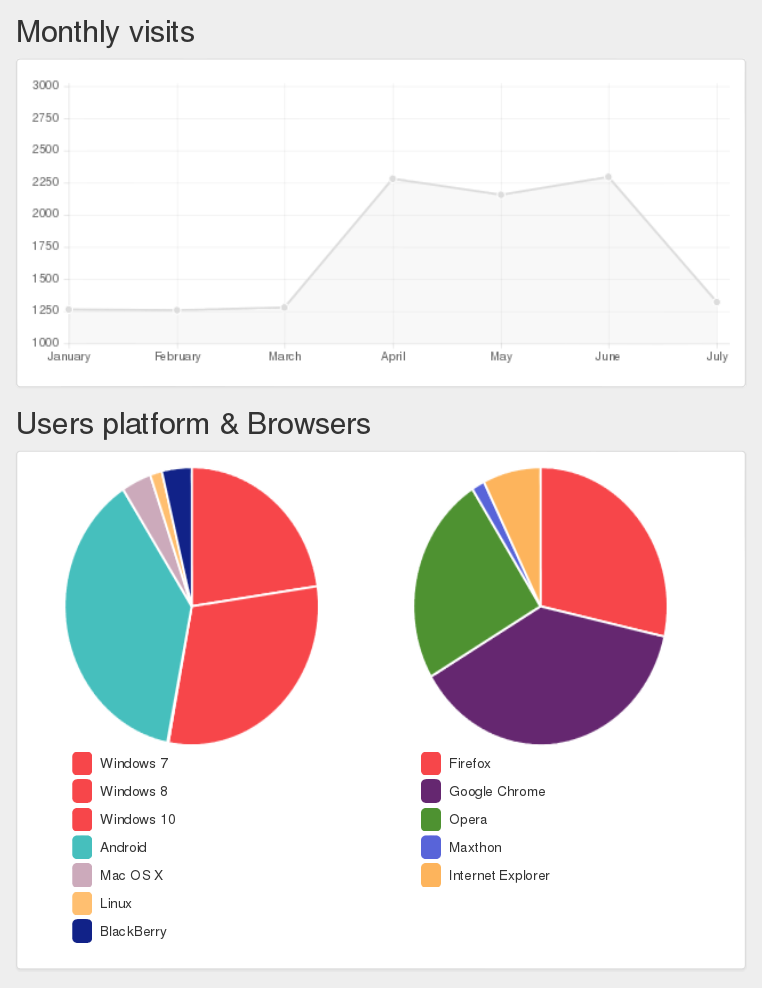
\includegraphics[width=10cm]{graphs}
          \caption{zobrazení dat o~návštěvnosti}
          \label{statistiky}
        \end{center}
      \end{figure}

      \begin{figure}[ht]
        \begin{center}
          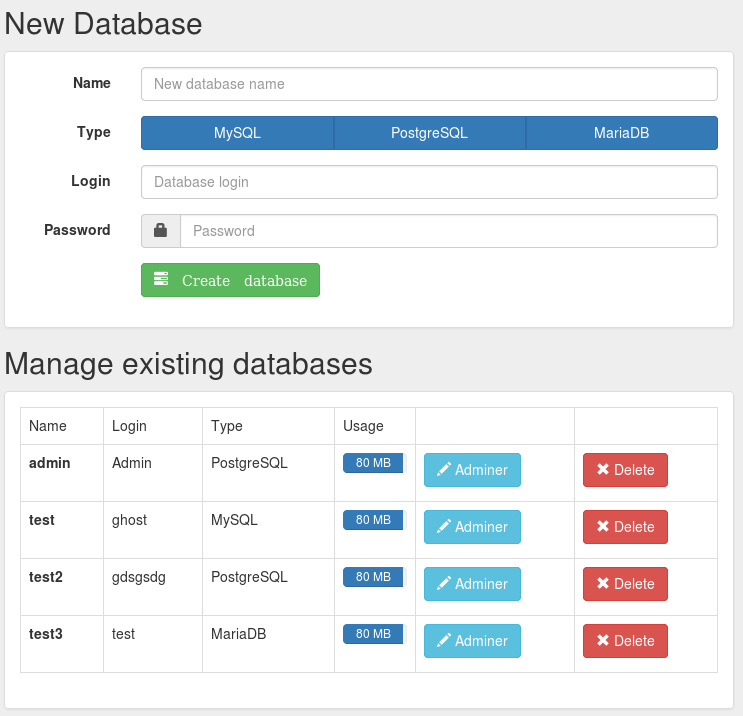
\includegraphics[width=10cm]{sql}
          \caption{nastavení SQL databáze}
        \end{center}
      \end{figure}

\end{document}
